% Generated by Sphinx.
\def\sphinxdocclass{report}
\documentclass[letterpaper,10pt,english]{sphinxmanual}
\usepackage[utf8]{inputenc}
\DeclareUnicodeCharacter{00A0}{\nobreakspace}
\usepackage[T1]{fontenc}
\usepackage{babel}
\usepackage{times}
\usepackage[Bjarne]{fncychap}
\usepackage{longtable}
\usepackage{sphinx}
\usepackage{multirow}


\title{Build a Site Event Calendar}
\date{December 31, 2011}
\release{0}
\author{Melissa Anderson}
\newcommand{\sphinxlogo}{}
\renewcommand{\releasename}{Release}
\makeindex

\makeatletter
\def\PYG@reset{\let\PYG@it=\relax \let\PYG@bf=\relax%
    \let\PYG@ul=\relax \let\PYG@tc=\relax%
    \let\PYG@bc=\relax \let\PYG@ff=\relax}
\def\PYG@tok#1{\csname PYG@tok@#1\endcsname}
\def\PYG@toks#1+{\ifx\relax#1\empty\else%
    \PYG@tok{#1}\expandafter\PYG@toks\fi}
\def\PYG@do#1{\PYG@bc{\PYG@tc{\PYG@ul{%
    \PYG@it{\PYG@bf{\PYG@ff{#1}}}}}}}
\def\PYG#1#2{\PYG@reset\PYG@toks#1+\relax+\PYG@do{#2}}

\def\PYG@tok@gd{\def\PYG@tc##1{\textcolor[rgb]{0.63,0.00,0.00}{##1}}}
\def\PYG@tok@gu{\let\PYG@bf=\textbf\def\PYG@tc##1{\textcolor[rgb]{0.50,0.00,0.50}{##1}}}
\def\PYG@tok@gt{\def\PYG@tc##1{\textcolor[rgb]{0.00,0.25,0.82}{##1}}}
\def\PYG@tok@gs{\let\PYG@bf=\textbf}
\def\PYG@tok@gr{\def\PYG@tc##1{\textcolor[rgb]{1.00,0.00,0.00}{##1}}}
\def\PYG@tok@cm{\let\PYG@it=\textit\def\PYG@tc##1{\textcolor[rgb]{0.25,0.50,0.56}{##1}}}
\def\PYG@tok@vg{\def\PYG@tc##1{\textcolor[rgb]{0.73,0.38,0.84}{##1}}}
\def\PYG@tok@m{\def\PYG@tc##1{\textcolor[rgb]{0.13,0.50,0.31}{##1}}}
\def\PYG@tok@mh{\def\PYG@tc##1{\textcolor[rgb]{0.13,0.50,0.31}{##1}}}
\def\PYG@tok@cs{\def\PYG@tc##1{\textcolor[rgb]{0.25,0.50,0.56}{##1}}\def\PYG@bc##1{\colorbox[rgb]{1.00,0.94,0.94}{##1}}}
\def\PYG@tok@ge{\let\PYG@it=\textit}
\def\PYG@tok@vc{\def\PYG@tc##1{\textcolor[rgb]{0.73,0.38,0.84}{##1}}}
\def\PYG@tok@il{\def\PYG@tc##1{\textcolor[rgb]{0.13,0.50,0.31}{##1}}}
\def\PYG@tok@go{\def\PYG@tc##1{\textcolor[rgb]{0.19,0.19,0.19}{##1}}}
\def\PYG@tok@cp{\def\PYG@tc##1{\textcolor[rgb]{0.00,0.44,0.13}{##1}}}
\def\PYG@tok@gi{\def\PYG@tc##1{\textcolor[rgb]{0.00,0.63,0.00}{##1}}}
\def\PYG@tok@gh{\let\PYG@bf=\textbf\def\PYG@tc##1{\textcolor[rgb]{0.00,0.00,0.50}{##1}}}
\def\PYG@tok@ni{\let\PYG@bf=\textbf\def\PYG@tc##1{\textcolor[rgb]{0.84,0.33,0.22}{##1}}}
\def\PYG@tok@nl{\let\PYG@bf=\textbf\def\PYG@tc##1{\textcolor[rgb]{0.00,0.13,0.44}{##1}}}
\def\PYG@tok@nn{\let\PYG@bf=\textbf\def\PYG@tc##1{\textcolor[rgb]{0.05,0.52,0.71}{##1}}}
\def\PYG@tok@no{\def\PYG@tc##1{\textcolor[rgb]{0.38,0.68,0.84}{##1}}}
\def\PYG@tok@na{\def\PYG@tc##1{\textcolor[rgb]{0.25,0.44,0.63}{##1}}}
\def\PYG@tok@nb{\def\PYG@tc##1{\textcolor[rgb]{0.00,0.44,0.13}{##1}}}
\def\PYG@tok@nc{\let\PYG@bf=\textbf\def\PYG@tc##1{\textcolor[rgb]{0.05,0.52,0.71}{##1}}}
\def\PYG@tok@nd{\let\PYG@bf=\textbf\def\PYG@tc##1{\textcolor[rgb]{0.33,0.33,0.33}{##1}}}
\def\PYG@tok@ne{\def\PYG@tc##1{\textcolor[rgb]{0.00,0.44,0.13}{##1}}}
\def\PYG@tok@nf{\def\PYG@tc##1{\textcolor[rgb]{0.02,0.16,0.49}{##1}}}
\def\PYG@tok@si{\let\PYG@it=\textit\def\PYG@tc##1{\textcolor[rgb]{0.44,0.63,0.82}{##1}}}
\def\PYG@tok@s2{\def\PYG@tc##1{\textcolor[rgb]{0.25,0.44,0.63}{##1}}}
\def\PYG@tok@vi{\def\PYG@tc##1{\textcolor[rgb]{0.73,0.38,0.84}{##1}}}
\def\PYG@tok@nt{\let\PYG@bf=\textbf\def\PYG@tc##1{\textcolor[rgb]{0.02,0.16,0.45}{##1}}}
\def\PYG@tok@nv{\def\PYG@tc##1{\textcolor[rgb]{0.73,0.38,0.84}{##1}}}
\def\PYG@tok@s1{\def\PYG@tc##1{\textcolor[rgb]{0.25,0.44,0.63}{##1}}}
\def\PYG@tok@gp{\let\PYG@bf=\textbf\def\PYG@tc##1{\textcolor[rgb]{0.78,0.36,0.04}{##1}}}
\def\PYG@tok@sh{\def\PYG@tc##1{\textcolor[rgb]{0.25,0.44,0.63}{##1}}}
\def\PYG@tok@ow{\let\PYG@bf=\textbf\def\PYG@tc##1{\textcolor[rgb]{0.00,0.44,0.13}{##1}}}
\def\PYG@tok@sx{\def\PYG@tc##1{\textcolor[rgb]{0.78,0.36,0.04}{##1}}}
\def\PYG@tok@bp{\def\PYG@tc##1{\textcolor[rgb]{0.00,0.44,0.13}{##1}}}
\def\PYG@tok@c1{\let\PYG@it=\textit\def\PYG@tc##1{\textcolor[rgb]{0.25,0.50,0.56}{##1}}}
\def\PYG@tok@kc{\let\PYG@bf=\textbf\def\PYG@tc##1{\textcolor[rgb]{0.00,0.44,0.13}{##1}}}
\def\PYG@tok@c{\let\PYG@it=\textit\def\PYG@tc##1{\textcolor[rgb]{0.25,0.50,0.56}{##1}}}
\def\PYG@tok@mf{\def\PYG@tc##1{\textcolor[rgb]{0.13,0.50,0.31}{##1}}}
\def\PYG@tok@err{\def\PYG@bc##1{\fcolorbox[rgb]{1.00,0.00,0.00}{1,1,1}{##1}}}
\def\PYG@tok@kd{\let\PYG@bf=\textbf\def\PYG@tc##1{\textcolor[rgb]{0.00,0.44,0.13}{##1}}}
\def\PYG@tok@ss{\def\PYG@tc##1{\textcolor[rgb]{0.32,0.47,0.09}{##1}}}
\def\PYG@tok@sr{\def\PYG@tc##1{\textcolor[rgb]{0.14,0.33,0.53}{##1}}}
\def\PYG@tok@mo{\def\PYG@tc##1{\textcolor[rgb]{0.13,0.50,0.31}{##1}}}
\def\PYG@tok@mi{\def\PYG@tc##1{\textcolor[rgb]{0.13,0.50,0.31}{##1}}}
\def\PYG@tok@kn{\let\PYG@bf=\textbf\def\PYG@tc##1{\textcolor[rgb]{0.00,0.44,0.13}{##1}}}
\def\PYG@tok@o{\def\PYG@tc##1{\textcolor[rgb]{0.40,0.40,0.40}{##1}}}
\def\PYG@tok@kr{\let\PYG@bf=\textbf\def\PYG@tc##1{\textcolor[rgb]{0.00,0.44,0.13}{##1}}}
\def\PYG@tok@s{\def\PYG@tc##1{\textcolor[rgb]{0.25,0.44,0.63}{##1}}}
\def\PYG@tok@kp{\def\PYG@tc##1{\textcolor[rgb]{0.00,0.44,0.13}{##1}}}
\def\PYG@tok@w{\def\PYG@tc##1{\textcolor[rgb]{0.73,0.73,0.73}{##1}}}
\def\PYG@tok@kt{\def\PYG@tc##1{\textcolor[rgb]{0.56,0.13,0.00}{##1}}}
\def\PYG@tok@sc{\def\PYG@tc##1{\textcolor[rgb]{0.25,0.44,0.63}{##1}}}
\def\PYG@tok@sb{\def\PYG@tc##1{\textcolor[rgb]{0.25,0.44,0.63}{##1}}}
\def\PYG@tok@k{\let\PYG@bf=\textbf\def\PYG@tc##1{\textcolor[rgb]{0.00,0.44,0.13}{##1}}}
\def\PYG@tok@se{\let\PYG@bf=\textbf\def\PYG@tc##1{\textcolor[rgb]{0.25,0.44,0.63}{##1}}}
\def\PYG@tok@sd{\let\PYG@it=\textit\def\PYG@tc##1{\textcolor[rgb]{0.25,0.44,0.63}{##1}}}

\def\PYGZbs{\char`\\}
\def\PYGZus{\char`\_}
\def\PYGZob{\char`\{}
\def\PYGZcb{\char`\}}
\def\PYGZca{\char`\^}
\def\PYGZsh{\char`\#}
\def\PYGZpc{\char`\%}
\def\PYGZdl{\char`\$}
\def\PYGZti{\char`\~}
% for compatibility with earlier versions
\def\PYGZat{@}
\def\PYGZlb{[}
\def\PYGZrb{]}
\makeatother

\begin{document}

\maketitle
\tableofcontents
\phantomsection\label{index::doc}



\chapter{Build a Site Event Calendar}
\label{event_calendar::doc}\label{event_calendar:build-a-site-event-calendar}

\section{Ingredients}
\label{event_calendar:ingredients}

\subsection{Staple}
\label{event_calendar:staple}\begin{enumerate}
\item {} 
\href{http://drupal.org/project/ctools}{http://drupal.org/project/ctools} - Enable Chaos tools

\item {} 
\href{http://drupal.org/project/views}{http://drupal.org/project/views} - Views: Enable Views and Views UI

\item {} 
\href{http://drupal.org/project/date}{http://drupal.org/project/date} - Date: Enable Date, Date API, Date Repeat, Date Popup

\item {} 
\href{http://drupal.org/project/fullcalendar}{http://drupal.org/project/fullcalendar} - FullCalendar: Enable FullCalendar, FullCalendar Colors

\item {} 
\href{http://drupal.org/project/colorsrs}{http://drupal.org/project/colorsrs} API - Other: Enable Colors (install the dev version)

\item {} 
\href{http://drupal.org/project/colorboxbox}{http://drupal.org/project/colorboxbox} - Other: Enable Colorbox

\end{enumerate}

\textbf{Drush users:}

\begin{Verbatim}[commandchars=\\\{\}]
drush dl ctools views date date\_api fullcalendar fullcalendar\_colors colors colorbox
drush en ctools views views\_ui date date\_api date\_repeat date\_popup
fullcalendar fullcalendar\_colors colors colorbox -y
\end{Verbatim}


\subsection{Specialty}
\label{event_calendar:specialty}
FullCalendar JQuery Libraries
\begin{enumerate}
\item {} 
Visit \href{http://arshaw.com/fullcalendar}{http://arshaw.com/fullcalendar}

\item {} 
Download the most recent version of the plugin.

\item {} 
Unzip fullcalendar/fullcalendar to sites/all/libraries/fullcalendar (e.g., sites/all/libraries/fullcalendar/fullcalendar.min.js).

\item {} 
Do no include the demos or jQuery directories.

\end{enumerate}

ColorBox Library
\begin{enumerate}
\item {} 
Visit \href{http://jacklmoore.com/colorbox/}{http://jacklmoore.com/colorbox/}

\item {} 
Download Current version

\item {} 
Unzip it straight into sites/all/libraries (e.g., sites/all/libraries/colorbox)

\end{enumerate}


\section{Part 1: Build a way to create events}
\label{event_calendar:part-1-build-a-way-to-create-events}

\subsection{1.1: Add a new content type called Event}
\label{event_calendar:add-a-new-content-type-called-event}
\emph{Structure \textgreater{} Content types \textgreater{} +Add new content type}

Name: Event

Description: Create an event for display on the site calendar

\begin{tabulary}{\linewidth}{|L|L|}
\hline

Submission Form Settings
 & 
Title field label: Event
\\\hline

Publishing Options
 & 
{[}√{]} Published (Check only this option; uncheck others)
\\\hline

Display Settings
 & 
{[} {]} Display author and date information (Uncheck this)
\\\hline

Comment Settings
 & 
Closed (Select Closed)
\\\hline

Menu Settings
 & 
{[} {]} Uncheck all menus
\\\hline
\end{tabulary}



\subsection{1.2: Configure Region and Language Settings}
\label{event_calendar:configure-region-and-language-settings}
\emph{Configuration \textgreater{} Regional and language \textgreater{} Regional settings}

The module and status pages will show warnings and display instructions for initially configuring Date module.

Regional Settings
Locale
\begin{enumerate}
\item {} 
Default country: United States

\item {} 
First day of the week: Sunday

\item {} 
{[} {]} Use ISO-8601 week numbers  (Leave unchecked)

\end{enumerate}

Time Zones

For this recipe, the calendar represents events happening in a single geographical location, so we won't be using timezone settings.
\begin{enumerate}
\item {} 
Default time zone: America/Los Angeles

\item {} 
{[} {]} Users may set their own timezones (Uncheck this)

\end{enumerate}


\subsection{1.3 Configure Date and Time}
\label{event_calendar:configure-date-and-time}
\emph{Configuration \textgreater{} Regional and language \textgreater{} Date and time}

Initial Date Module Configuration
\begin{enumerate}
\item {} 
Select formats for Long, Medium, or Short (Accept the defaults)

\item {} 
Click Save configuration. This provides the initial configuration for the date module and removes the warning on the modules page.

\end{enumerate}

Add a new date format
\begin{enumerate}
\item {} 
Choose the Formats tab (upper right)

\item {} 
+Add format

\item {} 
Format string: d M Y

\item {} 
Save with: Add format

\item {} 
Choose the Types tab (upper right)

\item {} 
+Add date type

\item {} 
Date type: Block-short \textless{}- this is just a label, you can choose any formatting you like.

\item {} 
Date format: Choose the example of the new format from the bottom of the select list: 14 Nov 2011

\item {} 
Save with: Add date type

\end{enumerate}

Note: If you make a mistake with the format but don't notice until later, you can edit a date format by returning to \emph{Configuration \textgreater{} Regional and Language: Date and Time \textgreater{} Formats} and clicking the edit link for the format in question. Unfortuantely this will cause the format to be unassigned from its Date type. Visit the Types tab and re-select the format from the dropdown list where appropriate.  If you forget this last step, the date field won't be automatically updated throughout your site.


\subsection{1.4: Add a date field}
\label{event_calendar:add-a-date-field}
Structure \textgreater{} Content types \textgreater{} Event \textgreater{} Manage fields
Add new field
\begin{enumerate}
\item {} 
Label: Date

\item {} 
Field name: date

\item {} 
Type of data to store: Date \textless{}- plain Date, not the ISO or Unix format

\item {} 
Form element to edit the data: Popup calendar with repeat options

\end{enumerate}

Field Settings
\begin{enumerate}
\item {} 
Date attributes to collect

\item {} 
{[}√{]} Check Collect an end date

\item {} 
{[}√{]} Required field

\item {} 
Accept other default field settings

\item {} 
Save.

\end{enumerate}

Event Settings
\begin{enumerate}
\item {} 
{[}√{]} Check Collect an end date

\item {} 
Accept the rest as is.

\item {} 
Save settings.

\end{enumerate}


\subsection{1.5: Rarrange the items in a way that makes sense}
\label{event_calendar:rarrange-the-items-in-a-way-that-makes-sense}
\emph{Structure \textgreater{} Content types \textgreater{} Event \textgreater{} Manage fields}

Use the grabber to drag and drop the fields into order:
\begin{enumerate}
\item {} 
Event name

\item {} 
Date

\item {} 
Body

\item {} 
URL path settings.

\end{enumerate}

Remember to Save.


\subsection{1.6: Create proper paths}
\label{event_calendar:create-proper-paths}
\emph{Configuration \textgreater{} Search and Metadata: URL aliases \textgreater{} Patterns}

Later on, we'll be creating a landing page at /calendar, so we're adding that to the path now.
\begin{enumerate}
\item {} 
Pattern for all Event paths: calendar/{[}node:title{]}

\end{enumerate}


\subsection{1.7: Create an event}
\label{event_calendar:create-an-event}
\emph{Content \textgreater{} +Add content}
\begin{enumerate}
\item {} 
Add an event on today called Training

\item {} 
Check that the path is as you expected, e.g. \href{http://eventcalendar.everydaydrupal.com/calendar/training-opensourcery}{http://eventcalendar.everydaydrupal.com/calendar/training-opensourcery}

\end{enumerate}


\section{Part 2: Create the calendar}
\label{event_calendar:part-2-create-the-calendar}

\subsection{2.1: Add a calendar view}
\label{event_calendar:add-a-calendar-view}
\emph{Structure \textgreater{} Views \textgreater{} +Add new view}
\begin{enumerate}
\item {} 
View name: Calendar

\item {} 
Show content of type Event sorted by Unsorted

\item {} 
{[}√{]} Create a page

\item {} 
Page title: Calendar

\item {} 
Path: calendar

\item {} 
Display format: FullCalendar

\item {} 
Items to display: (ignore)

\item {} 
{[}  {]} Use pager

\item {} 
{[}√{]} Create menu link:Menu: Main menuLink text: Event calendar

\item {} 
{[}√{]} Include an RSS feed

\item {} 
Feed path: calendar.xml

\item {} 
Continue \& edit

\end{enumerate}


\subsubsection{2.1.1 Add the date field}
\label{event_calendar:add-the-date-field}
You'll see an error message as soon as you've clicked Continue \& edit. You have to add the Date field from your event to the view for the calendar to function.

In the fields section of the left-hand column:

Fields
\begin{enumerate}
\item {} 
add:

Content: Date
Appears in: node:event.

\item {} 
{[} {]} Remove the check in the box Create a label

\item {} 
It's your choice what you set in the other visible areas. Don't change anything in the collapsed field groups.

\item {} 
Apply (All displays)

\end{enumerate}


\subsubsection{2.1.2 Advanced}
\label{event_calendar:advanced}
Other

For the drag and drop functionality to work when you switch pages, you MUST expancd the Advanced fieldgroup and set Ajax to Yes.


\subsubsection{2.1.3 Configure the feed}
\label{event_calendar:configure-the-feed}
We want a feed icon to appear on the page with the calendar so that feed users can find the feed URL.

If you create the feed on the initial set screen, this will be set up automatically, but if you create the feed later, you'll need to set it up manually.

In the center column of the view's Feed display, under Feed settings, choose:
\begin{quote}

Attach to:

{[}√{]} Master

{[}√{]} Page
\end{quote}


\section{Part 3: Create and place an Upcoming events block}
\label{event_calendar:part-3-create-and-place-an-upcoming-events-block}
We'll create an Upcoming events block for the front page and our calendar pages. We could build this in the same view as the calendar, but since it's substantially different, we'll create it in its own view.


\subsection{3.1: Create the block}
\label{event_calendar:create-the-block}
\emph{Structure \textgreater{} Views \textgreater{} +Add new view}
\begin{enumerate}
\item {} 
View name: Upcoming events

\item {} 
Show content of type Event sorted by Unsorted \textless{}- Choosing Newest first here would sort by when the Event node was created, not when the event was scheduled.

\item {} 
{[} {]} Create a page

\item {} 
{[}√{]} Create a block

\item {} 
Display fomat: Unformatted list of fields

\item {} 
Continue \& Edit

\end{enumerate}


\subsubsection{3.1.1 Add the date field}
\label{event_calendar:id1}
Fields
\begin{enumerate}
\item {} 
add:

\item {} 
Content: Date

\item {} 
Appears in: node:event.

\item {} 
{[} {]} Remove the check in the box Create a label (Remove check)

\item {} 
{[} {]} Exclude from display (Leave unchecked)

\item {} 
Formatter:

\item {} 
Date and time

\item {} 
Choose how users view dates and times:

\item {} 
Block-short

\item {} 
Display: Both Start and End dates

\item {} 
Don't change anything in the collapsed field groups.

\item {} 
Apply (All displays)

\end{enumerate}


\subsubsection{3.1.2 Filter to future dates}
\label{event_calendar:filter-to-future-dates}
I filter on the date an event ends so that it remains visible while it's happening, allowing users to reference directions or other information quickly. You might choose to filter by the Start date if it better suits your needs.

Filter Criteria
\begin{enumerate}
\item {} 
add:

\item {} 
Content: Date - end date (field\_date:value2)

\item {} 
Configure extra settings for filter criterion:

\item {} 
Accept the defaults. They won't matter.

\item {} 
Configure filter criterion:

\item {} 
Operator:

\item {} 
Is greater than

\item {} 
Enter a relative date

\item {} 
Relative date:

\item {} 
now

\end{enumerate}


\subsubsection{3.1.3 Sort by date}
\label{event_calendar:sort-by-date}\begin{enumerate}
\item {} 
add:

\item {} 
Content: Date - start date (field\_date)

\item {} 
Click Add and configure

\item {} 
Choose Sort ascending (default)

\item {} 
Apply

\item {} 
Don't forget to save the view, too!

\end{enumerate}


\subsection{3.3 Place the block}
\label{event_calendar:place-the-block}
\emph{Structure \textgreater{} Blocks \textgreater{} Views: Upcoming Event \textgreater{} Configure}

Block title:Upcoming events
\begin{description}
\item[{Region Settings:}] \leavevmode
Bartik (default theme)
Sidebar Second

\end{description}

\begin{tabular}{|p{0.475\linewidth}|p{0.475\linewidth}|}
\hline
 \multicolumn{2}{|l|}{\textbf{
Visibility Settings
}}\\\hline

Pages
 & 
◉ Only the listed pages (Select this, enter the text below)
\begin{itemize}
\item {} 
\textless{}front\textgreater{}

\item {} 
calendar/*

\end{itemize}
\\\hline

Content types
 & 
{[}√{]} Gallery (Check only this option)
\\\hline

Roles
 & 
(Leave as is)
\\\hline

Users
 & 
(Leave as is)
\\\hline
\end{tabular}



\section{Part 4: Categorize events by terms}
\label{event_calendar:part-4-categorize-events-by-terms}

\subsection{4.1 Create the vocabulary and add terms to it}
\label{event_calendar:create-the-vocabulary-and-add-terms-to-it}
\emph{Structure \textgreater{} Taxonomy \textgreater{} +Add vocabulary}
\begin{enumerate}
\item {} 
Name: Event Types

\item {} 
Description: Categorize events by type.

\item {} 
Add two terms (for the Category Event Types

\item {} 
Name: Public

\item {} 
Description: These events are open to the public

\item {} 
Accept the rest of the defaults and save.

\item {} 
Name: Staff Meeting

\item {} 
Description: These meetings are required meetings for all staff.

\item {} 
Accept the rest of the defaults and save.

\end{enumerate}


\subsection{4.2 Add the term to the Event content type}
\label{event_calendar:add-the-term-to-the-event-content-type}
\emph{Structure \textgreater{} Content Types \textgreater{} Event \textgreater{} Manage Fields}
\begin{enumerate}
\item {} 
Add new field

\item {} 
LABEL: Add new field: Event type

\item {} 
NAME: field\_event\_type

\item {} 
FIELD: Term reference

\item {} 
WIDGET: Select List

\item {} 
Save

\item {} 
Make sure the Event Types category is selected.

\item {} 
Save field settings

\item {} 
Accept all the defaults

\item {} 
Save settings

\item {} 
Drag the Event Type term beneath the Event name.

\item {} 
Save.

\end{enumerate}


\subsection{4.3 Create and tag events}
\label{event_calendar:create-and-tag-events}
\emph{Content \textgreater{} +Add Content}
\begin{enumerate}
\item {} 
Create an event in the current month tagged Public

\item {} 
Create an event in the current month tagged Staff Meeting

\item {} 
Create an event in the current month and don't tag it.

\end{enumerate}


\section{Part 5: Color code events}
\label{event_calendar:part-5-color-code-events}
\emph{Configuration \textgreater{} User Interface: FullCalendar \textgreater{} Colors (tab) \textgreater{} Taxonomy (subtab)}

You can color code your events by Node Type, Taxonomy, or User Role.


\subsection{5.1 Set the default color}
\label{event_calendar:set-the-default-color}\begin{enumerate}
\item {} 
Choose the color for events that aren't labeled with a term.

\end{enumerate}


\subsection{5.2 Set the colors for the taxonomy terms}
\label{event_calendar:set-the-colors-for-the-taxonomy-terms}\begin{enumerate}
\item {} 
Expand Event types.

\item {} 
Use the color picker to assign different colors.

\item {} 
Save configuration

\end{enumerate}


\subsection{5.3 Check out the colors. Try dragging. Try dropping.}
\label{event_calendar:check-out-the-colors-try-dragging-try-dropping}

\section{Part 6: Create filters based on your categories}
\label{event_calendar:part-6-create-filters-based-on-your-categories}
There are several ways to maintain a master calendar and then filter it so that you show only certain events.

First, we'll add a filter to the main calendar so users can choose what to see.


\subsection{6.1: Add drop down filter to the existing calendar}
\label{event_calendar:add-drop-down-filter-to-the-existing-calendar}
\emph{Structure \textgreater{} Views}
\begin{enumerate}
\item {} 
Locate your calendar on the main views page or use the contextual links while viewing it to edit.

\item {} 
Filter Criteria

add
Choose Content: Has taxonomy term

\item {} 
Add and configure filter criteria

\item {} 
For This page (override)

\item {} 
{[}  {]} Expose this filter to visitors, to allow them to change it

\item {} 
Label: Choose a category

\item {} 
Apply (this display)

\end{enumerate}


\subsection{6.2 Create a pre-filtered option}
\label{event_calendar:create-a-pre-filtered-option}
We're going to filter the calendar so that it only shows one kind of event and the user cannot change this. Organizations with complex structures  may prefer to shield their users from the selection porcess and choose instead to place these calendars in department areas.
\begin{enumerate}
\item {} 
Clone the page display

\item {} 
Change the Display name to ``Filtered by Page'' for your own convenience

\item {} 
Path: calendar/\%

\item {} 
Advanced

\item {} 
Contextual Filters

add
Content: Has taxonomy term ID

\item {} 
In the configuration for the filter:

\item {} 
For: This page (override)

\item {} 
When the filter value is NOT in the URL

◉ Provide default value
Type: Taxonomy term ID from URL \textless{}- Choose from the select list.

\item {} 
{[} {]} Uncheck Load default filter from term page

\item {} 
Click Add (This Display). Note: If the button says Apply (all displays), you missed step 1. You can make that change now.

\end{enumerate}

You might wonder why we've created a second display instead of just adding the contextual filter to the first Page display and putting the \% wildcard at the end of its Path.

The wildcard prevents putting the calendar on the menu, so we had a choice. We could add all of the calendar links to the menu manually and create a single display, or we can create the main display and duplicate it. I chose the second because I wanted the main calendar view to contain the drop down filter that I did not want to place on the other views.


\subsection{6.3 Add our filtered views to the main menu}
\label{event_calendar:add-our-filtered-views-to-the-main-menu}
\emph{Structure \textgreater{} Menus \textgreater{} Main Menu \textgreater{} add link}

Because we're working with a simple test site, we'll add menu entries for our event types to the main menu. If you need to verify the taxonomy id of a term you can Structure \textgreater{} Taxonomy \textgreater{} Event Types, list terms, and the Term ID is visible in the URL of the edit link (taxonomy/term/\#)
\begin{enumerate}
\item {} 
Menu link title: Public Events

\item {} 
Path: calendar/1

\item {} 
Save

\item {} 
+Add link

\item {} 
Menu link title: Staff Meetings

\item {} 
Path: calendar/2

\item {} 
Save

\end{enumerate}

\textbf{Using terms vs. term names:} Term names are better, really, because they're more memorable. If the name is changed, however, then all the links using the name have to be updated or redirects must be put into place.


\section{Part 7: Set and test permissions}
\label{event_calendar:part-7-set-and-test-permissions}
\emph{People \textgreater{} Permissions}

If you are not using the Test Kitchen Install Profile or if you are new to the idea of users, roles, permissions or masquerade, see \href{http://training.opensourcery.com/basics}{http://training.opensourcery.com/basics}


\subsection{7.1 Set permissions}
\label{event_calendar:set-permissions}
Set permissions as follows:

\begin{tabulary}{\linewidth}{|L|L|L|}
\hline
\textbf{
Author
} & \textbf{
Editor
} & \textbf{
Admin
}\\\hline

{[}√{]} Event: Create new content
 & 
{[}√{]} Event: Create new content
 & 
{[}√{]} Event: Create new content
\\\hline

{[}√{]}  Event: Edit own content
 & 
{[} {]} Event: Edit own content
 & 
{[}√{]} Event: Edit own content
\\\hline

{[} {]}  Event: Edit any content
 & 
{[}√{]} Event: Edit any content
 & 
{[}√{]} Event: Edit any content
\\\hline

{[}√{]}  Event: Delete own content
 & 
{[} {]} Event: Delete own content
 & 
{[}√{]} Event: Delete own content
\\\hline

{[} {]}  Event: Delete any content
 & 
{[}√{]}  Event: Delete any content
 & 
{[}√{]} Event: Delete any content
\\\hline
\end{tabulary}



\subsection{7.2 Test Author privileges}
\label{event_calendar:test-author-privileges}
Masquerade as Test Author and ensure you CAN:
\begin{enumerate}
\item {} 
Create an Event

\item {} 
Edit that Event

\item {} 
Delete that Event

\end{enumerate}

Ensure you CANNOT:
\begin{enumerate}
\item {} 
Edit galleries you didn’t create

\item {} 
Delete galleries you didn’t create

\end{enumerate}

When you’re done, remember to Switch back


\subsection{7.3 Test Editor privileges}
\label{event_calendar:test-editor-privileges}
Masquerade as Test Editor and ensure you CAN:
\begin{enumerate}
\item {} 
Create an Event

\item {} 
Edit that Event

\item {} 
Delete that Event

\item {} 
Edit an Event you didn’t create

\item {} 
Delete an Event you didn’t create

\end{enumerate}


\chapter{Build Image Galleries and Slideshows}
\label{slides:build-image-galleries-and-slideshows}\label{slides::doc}
Create photo galleries that elegantly display photos and titles with optional slide show viewing controls. Upload an image just once and have a variety of high quality sizes created without ever opening a graphics program. Then, bring them all together into a beautiful index that groups them by category!

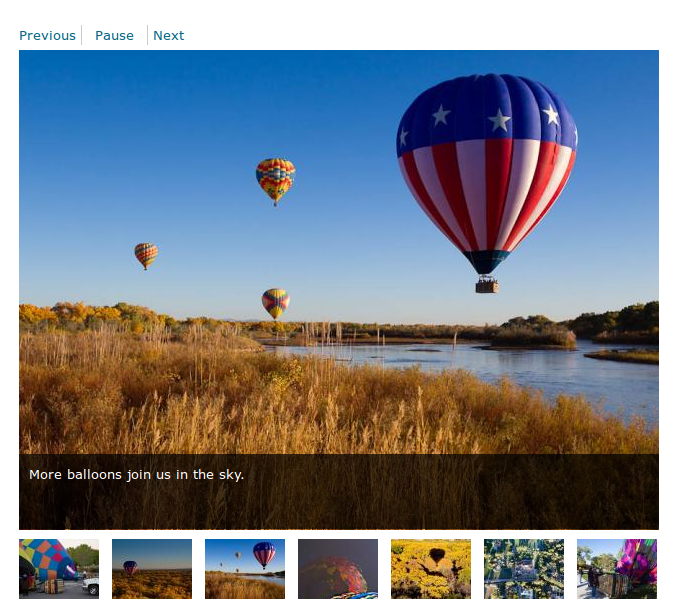
\includegraphics{balloons.png}


\section{Ingredients}
\label{slides:ingredients}

\subsection{Staple}
\label{slides:staple}\begin{enumerate}
\item {} 
\href{http://drupal.org/project/ctools}{http://drupal.org/project/ctools} - Enable Chaos Tools (all others are not needed)

\item {} 
\href{http://drupal.org/project/views}{http://drupal.org/project/views} - Enable Views and Views UI

\item {} 
\href{http://drupal.org/project/libraries}{http://drupal.org/project/libraries} - Enable Libraries

\item {} 
\href{http://drupal.org/project/views\_slideshow}{http://drupal.org/project/views\_slideshow} - Enable Views Slideshow

\end{enumerate}

\textbf{Drush users:}

\begin{Verbatim}[commandchars=\\\{\}]
drush dl ctools views libraries views\_slideshow
drush en ctools views views\_ui libraries views\_slideshow views\_slideshow\_cycle -y
\end{Verbatim}


\subsection{Speciality}
\label{slides:speciality}
Views Slideshow module uses two external libraries.

Required for basic slide show functionality:
\begin{enumerate}
\item {} 
Visit \href{http://malsup.com/jquery/cycle/download.html}{http://malsup.com/jquery/cycle/download.html}

\item {} 
Click the link to “Cycle Plugin”

\item {} 
In your browser, choose File \textgreater{} Save Page as \textgreater{} jquery.cycle.all.js

\item {} 
Place in sites/all/libraries/jquery.cycle (you'll have to create that folder) so that the final path looks like sites/all/libraries/jquery.cycle/jquery.cycle.all.js

\end{enumerate}

Required for advanced features, which include setting the speed of the slide show:
\begin{enumerate}
\item {} 
Visit \href{https://github.com/douglascrockford/JSON-js/downloads}{https://github.com/douglascrockford/JSON-js/downloads} and download the appropriate format, .zip or .tar.gz, for your environment.

\item {} 
Extract it

\item {} 
Rename the directory (which begins with douglascrockford-) to json2

\item {} 
Place it in sites/all/libraries so that the final path looks like: sites/all/libraries/json2/json2.js

\end{enumerate}


\section{Part 1: Build the form for creating galleries}
\label{slides:part-1-build-the-form-for-creating-galleries}

\subsection{1.1: Add a new content type called Gallery}
\label{slides:add-a-new-content-type-called-gallery}
\emph{Structure \textgreater{} Content types \textgreater{} +Add new content type}

Name: Gallery

Description: Create an image gallery with slide show controls.

\begin{tabulary}{\linewidth}{|L|L|}
\hline

Submission Form Settings
 & 
Title field label: Gallery name
\\\hline

Publishing Options
 & 
{[}√{]} Published (Check only this option; uncheck others)
\\\hline

Display Settings
 & 
{[} {]}  Display author and date information (Uncheck this)
\\\hline

Comment Settings
 & 
Closed (Select Closed)
\\\hline

Menu Settings
 & 
{[} {]}  Uncheck all menus
\\\hline
\end{tabulary}



\subsection{1.2: Add an image field}
\label{slides:add-an-image-field}
\emph{Structure \textgreater{} Content types \textgreater{} Gallery \textgreater{} Manage fields}


\subsubsection{Add new field}
\label{slides:add-new-field}\begin{enumerate}
\item {} 
Label: Gallery Image

\item {} 
Field name: gallery\_image

\item {} 
Type of data to store: Image

\item {} 
Form element to edit the data: Image \textless{}- the default

\item {} 
Save

\end{enumerate}


\subsubsection{Field Settings}
\label{slides:field-settings}
Leave as is: Public files selected, no default image


\subsubsection{Gallery Settings}
\label{slides:gallery-settings}
There are a lot of settings here! Accept the defaults EXCEPT the following:

File directory: galleries

Minimum image resolution: 640 x 480

We’re building our gallery around a common 640 x 480 resolution. By requiring images to be at least that large here, we can prevent jarring changes in size and eliminate white space between main images and thumbnails.

{[}√{]} Enable Title field


\subsubsection{Gallery Image Field Settings}
\label{slides:gallery-image-field-settings}
Number of values: Unlimited


\subsection{1.3: Create proper paths}
\label{slides:create-proper-paths}
\emph{Configuration \textgreater{} Search and Metadata: URL aliases \textgreater{} Patterns}

Later on, we’ll be creating a landing page at /galleries, so we’re adding that to the path now.

Pattern for all Gallery paths: galleries/{[}node:title{]}


\subsection{1.4: Create a test gallery}
\label{slides:create-a-test-gallery}
\emph{Content \textgreater{} +Add content \textgreater{} Gallery}
\begin{enumerate}
\item {} 
Gallery name: Test Gallery

\item {} 
Body text: Optional

\item {} 
Browse and upload at least 4 images, giving each one a title.

\item {} 
Check the URL pattern is what you expect, something like: \href{http://tests.l/galleries/test-gallery}{http://tests.l/galleries/test-gallery}

\end{enumerate}


\subsection{1.5: Hide the default display of images}
\label{slides:hide-the-default-display-of-images}
\emph{Structure \textgreater{} Content types \textgreater{} Gallery \textgreater{} Manage display}
\begin{enumerate}
\item {} 
Set the Default display setting format for Image to Hidden.

\item {} 
Verify the Teaser display format is hidden. It should already be set that way.

\item {} 
Go to Content and view the gallery you created in 1.4

\item {} 
You should see nothing but body text you entered.

\end{enumerate}


\section{Part 2: Create custom image sizes}
\label{slides:part-2-create-custom-image-sizes}

\subsection{2.1: Main gallery image}
\label{slides:main-gallery-image}
\emph{Configuration \textgreater{} Media \textgreater{} Image styles \textgreater{} +Add style}

We set a minimum resolution for uploading the image, but users can upload higher resolution if the wish. Using this style ensures uniform presentation within the gallery.
\begin{enumerate}
\item {} 
Image style name: gallery\_main

\item {} 
In Effect, select the new effect Scale and crop from the drop down, then click Add

\item {} 
Width: 640

\item {} 
Height: 480

\item {} 
Click the Add effect button (Your changes are saved; the button on the next page is just for reordering the effects if there is more than one.)

\end{enumerate}


\subsection{2.2: Gallery thumbnails}
\label{slides:gallery-thumbnails}
\emph{Configuration \textgreater{} Media \textgreater{} Image styles \textgreater{} +Add style}

The thumbnail settings are chosen so the images stay proportional to an 640 x 480 main image and so seven thumbnails fit width-wise underneath it, with an allowance for padding.
\begin{enumerate}
\item {} 
Image style name: gallery\_thumb

\item {} 
In Effect, choose Scale and crop, then click Add

\item {} 
Width: 80

\item {} 
Height: 60

\item {} 
Click the Add effect button

\end{enumerate}


\subsection{2.3: Gallery index thumbnails}
\label{slides:gallery-index-thumbnails}
\emph{Configuration \textgreater{} Media \textgreater{} Image styles \textgreater{} +Add style}

Add a third style for the index of galleries on the site.
\begin{enumerate}
\item {} 
Click +Add style again

\item {} 
Image style name: gallery\_index

\item {} 
In Effect, choose Scale and crop, then click Add

\item {} 
Width: 160

\item {} 
Height: 120

\item {} 
Click the Add effect button

\end{enumerate}


\section{Part 3: Create the galleries}
\label{slides:part-3-create-the-galleries}
Views delivers extraordinary power to the non-programmer, and the price is a densely-packed interface. We describe the steps below, but there's a place where the screen cast is worth a thousand words!


\subsection{3.1: Create the actual gallery display}
\label{slides:create-the-actual-gallery-display}
\emph{Structure \textgreater{} Views \textgreater{} +Add new view}

On the introductory Views page:
\begin{figure}[htbp]
\centering

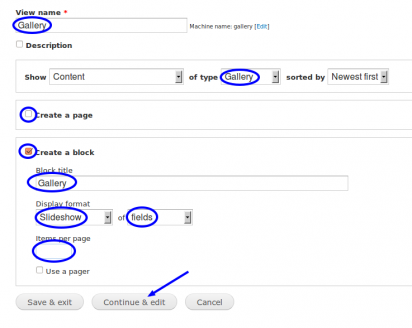
\includegraphics[width=0.650\linewidth]{slideshow-3.1-412x328.png}
{\small \begin{enumerate}
\item {} 
View name: Gallery

\item {} 
Show content of type Gallery sorted by Newest first

\item {} 
{[} {]}    Uncheck Page

\item {} 
{[}√{]}  Check Block

\item {} 
Block title: Gallery

\item {} 
Display fomat: Slideshow of fields

\item {} 
Items per page: (Make this blank)

\item {} 
Continue \& Edit

\end{enumerate}
}\end{figure}
\begin{figure}[htbp]
\centering

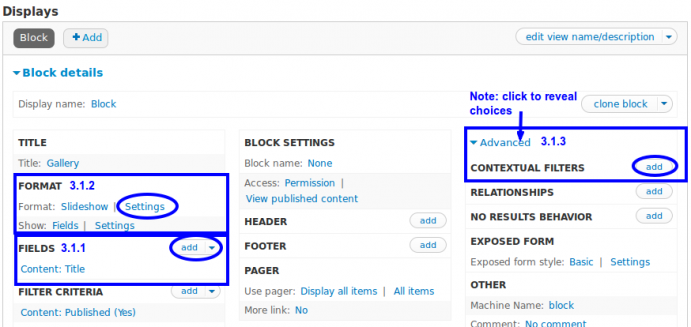
\includegraphics[width=0.650\linewidth]{slideshow-3.1-main.png}
{\small 
In main Views interface, we'll configure three areas:

\begin{DUlineblock}{0em}
\item[] 3.1.1 - available fields
\item[] 3.1.2 - row style settings,
\item[] 3.1.3 - the contextual filter.
\end{DUlineblock}

We’ll set them up in this order because they depend upon each other, even though they’re visually in a different order.
}\end{figure}


\subsubsection{3.1.1: Add Fields}
\label{slides:add-fields}
First, add the main gallery image:
\begin{enumerate}
\item {} 
Fields: add

\item {} 
From the popup, select: Content: Gallery image

\item {} 
{[} {]} Remove the check in the box Create a label

\item {} 
Set the Image style to gallery\_main.

\item {} 
Multiple Field Values: {[} {]} Uncheck Display all values in the same row

\item {} 
Apply (All displays)

\end{enumerate}

Second, add the thumbnail gallery images. Much like the first step:
\begin{enumerate}
\item {} 
Fields: add

\item {} 
From the popup, select: Content: Gallery image

\item {} 
{[} {]} Remove the check in the box Create a label

\item {} 
{[}√{]} Check Exclude from display

\item {} 
Set the Image style to gallery\_thumb.

\item {} 
Multiple Field Values: {[} {]} Uncheck Display all values in the same row

\item {} 
Apply (All displays)

\end{enumerate}

Next, add the title.
\begin{enumerate}
\item {} 
Fields: add

\item {} 
From the popup, select:Content: Gallery image

\item {} 
{[} {]} Remove the check in the box Create a label

\item {} 
Leave other visible settings at their default

\item {} 
Multiple Field Values: {[} {]} Uncheck Display all values in the same row

\item {} 
Expand Rewrite Results

\item {} 
{[}√{]} Rewrite the output of this field

\item {} 
In the text field, enter {[}field\_gallery\_image\_2-title{]} (View the available patterns by expanding Replacement Patterns.)

\item {} 
Apply (all displays)

\end{enumerate}

You now have three fields, all named the same thing but configured differently: the main image, the thumbnails, and the image titles.

Finally, remove the Content Title since it redundantly displays the name of the gallery.
\begin{enumerate}
\item {} 
Click the link Content: Title

\item {} 
Scroll and click Remove

\end{enumerate}


\subsubsection{3.1.2: Format}
\label{slides:format}\begin{enumerate}
\item {} 
Format: Settings

\item {} 
In the Top Widgets section, check Controls.

\item {} 
In the Bottom Widgets section, check Pager and choose the middle instance of Content: Gallery Image. This will provide the thumbnail images for the pager.

\item {} 
Apply (All displays)

\end{enumerate}


\subsubsection{3.1.3: Advanced}
\label{slides:advanced}\begin{enumerate}
\item {} 
Contextual Filter (Add)

\item {} 
Content: Nid

\item {} 
◉ Provide a default value \textgreater{} Type: Content ID from URL

\item {} 
Apply (All displays)

\end{enumerate}

Be sure to save the view!


\subsection{3.2: Place and configure the block}
\label{slides:place-and-configure-the-block}
\emph{Structure \textgreater{} Blocks \textgreater{} Views: Galleries \textgreater{} Configure}

Configuring the block to display only on Gallery nodes prevents it from being called on a view, and listing it only on specific pages prevents it from appearing on the Edit tab.

Block title:  \textless{}none\textgreater{}

Region Settings
\begin{quote}

Footheme (default theme)
Content
\end{quote}

\textbf{Visibility Settings}

\begin{tabulary}{\linewidth}{|L|L|}
\hline

Pages
 & 
◉ Only the listed pages (Select this and enter the text below)
galleries*
\\\hline

Content types
 & 
{[}√{]} Gallery (Check only this option)
\\\hline

Roles
 & 
(Leave as is)
\\\hline

Users
 & 
(Leave as is)
\\\hline
\end{tabulary}



\section{Part 4: Create an index of all galleries}
\label{slides:part-4-create-an-index-of-all-galleries}
\emph{Structure \textgreater{} Views \textgreater{} +Add new view}

You could create the gallery index page in the same view as the gallery block by adding a Page display, but the settings are different enough that they don’t gain a lot by sharing defaults, so we’ll create this as a separate view.


\subsection{4.1: Add a new view}
\label{slides:add-a-new-view}

\subsubsection{Intro screen}
\label{slides:intro-screen}\begin{enumerate}
\item {} 
View name: Galleries

\item {} 
Show Content of type Gallery sorted by Newest first

\item {} 
{[}√{]}  Create a page

\item {} 
Page title: Galleries

\item {} 
Display format: Grid of fields

\item {} 
Items to display: 24

\item {} 
{[}√{]}  Create a menu link \textgreater{} Menu: Main menu, Weight: 1

\item {} 
Menu link title: Galleries

\item {} 
Continue \& edit

\end{enumerate}


\subsubsection{Fields}
\label{slides:fields}\begin{enumerate}
\item {} 
add

\item {} 
Gallery image

\item {} 
{[} {]} Uncheck Create a label

\item {} 
Formatter: Image (no change)

\item {} 
Image style: gallery\_index

\item {} 
Link image to: Content

\item {} 
Apply (all displays)

\end{enumerate}

Be sure to save the view!


\subsection{4.2: A brief detour}
\label{slides:a-brief-detour}
\emph{Structure \textgreater{} Blocks \textgreater{} Main menu: configure}

Footheme uses the block system to place menus, and the main menu is not enabled yet.

Region Settings
\begin{enumerate}
\item {} 
Footheme (default theme). Select Menu Bar.

\item {} 
Save block

\end{enumerate}


\subsection{4.3: Auto-generate galleries}
\label{slides:auto-generate-galleries}
\emph{Configuration \textgreater{} Development: Generate content}
\begin{enumerate}
\item {} 
{[}√{]} Gallery (Uncheck others)

\item {} 
Accept the rest of the defaults

\item {} 
Generate

\end{enumerate}


\section{Part 5: Style the Gallery}
\label{slides:part-5-style-the-gallery}
We'll apply some basic formatting to the galleries.


\subsection{5.1: Open footheme.css}
\label{slides:open-footheme-css}
You can edit your style sheet any way that is comfortable for you. If you need more support than the username and password for your sandbox, see Connecting to your sandbox with sFTP at \href{http://training.opensourcery.com/basics/sftp}{http://training.opensourcery.com/basics/sftp}


\subsection{5.2: Arrange thumbnails beneath the main image}
\label{slides:arrange-thumbnails-beneath-the-main-image}
\begin{Verbatim}[commandchars=\\\{\}]
/* Arrange the thumbnails beneath the main image */
.views-content-field-gallery-image \PYGZob{}
  float: left;
  padding-right: 13px;
\PYGZcb{}

.views-slideshow-cycle-main-frame-row-item \PYGZob{}
  padding: 5px 20px;
\PYGZcb{}

.views-slideshow-controls-bottom \PYGZob{}
  padding: 0 0 0 20px;
\PYGZcb{}
\end{Verbatim}


\subsection{5.3: Format the controls}
\label{slides:format-the-controls}
\begin{Verbatim}[commandchars=\\\{\}]
/* Format the controls */
.views-slideshow-controls-text \PYGZob{}
  padding-left: 20px;
\PYGZcb{}

.views-slideshow-controls-text span \PYGZob{}
  display:  block;
  float: left;
\PYGZcb{}

.views\_slideshow\_controls\_text\_resume,
.views\_slideshow\_controls\_text\_pause\PYGZob{}
  text-align: center;
  width: 55px;
  border-left: 1px solid \#ccc;
  border-right: 1px solid \#ccc;
  padding: 0 5px;
  margin: 0 5px;
\PYGZcb{}
\end{Verbatim}


\subsection{5.4 Place title text over the main image}
\label{slides:place-title-text-over-the-main-image}
\emph{Structure \textgreater{} Views \textgreater{} Gallery: edit}

Placing opaque text on a transparent background requires some special setup. If the text is placed inside the transparent container, it will inherit the transparency. Instead, it must be placed parallel to the container and positioned.
\begin{enumerate}
\item {} 
Edit the third instance of the filed content: Galley image

\item {} 
Expand REWRITE RESULTS and edit to match:

\begin{Verbatim}[commandchars=\\\{\}]
\textless{}div class="transparency"\textgreater{}\textless{}/div\textgreater{}
\textless{}div class="overlay"\textgreater{}[field\_gallery\_image\_2-title]\textless{}/div\textgreater{}
\end{Verbatim}

\item {} 
Apply (all displays)

\item {} 
Add the styling to footheme.css:

\begin{Verbatim}[commandchars=\\\{\}]
/* Overlay the text on the main image */
.views-field-field-gallery-image \PYGZob{}
  position: relative;
\PYGZcb{}

.transparency \PYGZob{}
  position: absolute;
  bottom: -10px;
  left: 0px;
  width: 640px;
  height: 75px;
  background: black;
  margin: 20px;
  filter:alpha(opacity=70);
  opacity: 0.7;
  -moz-opacity:0.7;
\PYGZcb{}

.overlay \PYGZob{}
  color: white;
  position: absolute;
  bottom : 0px;
  left: 0px;
  height: 75px;
  padding: 0 30px 0 30px;
\PYGZcb{}
\end{Verbatim}

\end{enumerate}


\section{Part 6: Set and test permissions}
\label{slides:part-6-set-and-test-permissions}
\emph{People \textgreater{} Permissions}

If you are not using the Test Kitchen Install Profile or if you are new to the idea of users, roles, permissions or masquerade, see \href{http://training.opensourcery.com/basics}{http://training.opensourcery.com/basics}


\subsection{6.1: Set permissions}
\label{slides:set-permissions}
Set permissions as follows:

\begin{tabulary}{\linewidth}{|L|L|L|}
\hline
\textbf{
Author
} & \textbf{
Editor
} & \textbf{
Admin
}\\\hline

{[}√{]} Gallery: Create new content
 & 
{[}√{]} Gallery: Create new content
 & 
{[}√{]} Gallery: Create new content
\\\hline

{[}√{]}  Gallery: Edit own content
 & 
{[} {]}  Gallery: Edit own content
 & 
{[}√{]} Gallery: Edit own content
\\\hline

{[} {]}   Gallery: Edit any content
 & 
{[}√{]} Gallery: Edit any content
 & 
{[}√{]} Gallery: Edit any content
\\\hline

{[}√{]}  Gallery: Delete own content
 & 
{[} {]}  Gallery: Delete own content
 & 
{[}√{]} Gallery: Delete own content
\\\hline

{[} {]}   Gallery: Delete any content
 & 
{[}√{]}  Gallery: Delete any content
 & 
{[}√{]} Gallery: Delete any content
\\\hline
\end{tabulary}



\subsection{6.2: Test Author privileges}
\label{slides:test-author-privileges}
Masquerade as Test Author and ensure you CAN:
\begin{enumerate}
\item {} 
Create a gallery

\item {} 
Edit that gallery

\item {} 
Delete that gallery

\end{enumerate}

Ensure you CANNOT:
\begin{enumerate}
\item {} 
Edit galleries you didn’t create

\item {} 
Delete galleries you didn’t create

\end{enumerate}

When you’re done, remember to Switch back


\subsection{6.3: Test Editor privileges}
\label{slides:test-editor-privileges}
Masquerade as Test Editor and ensure you CAN:
\begin{enumerate}
\item {} 
Create a gallery

\item {} 
Edit that gallery

\item {} 
Delete that gallery

\item {} 
Edit a gallery you didn’t create

\item {} 
Delete a gallery you didn’t create

\end{enumerate}


\chapter{Perfecting Permissions: Editorial Workflow}
\label{workbench::doc}\label{workbench:perfecting-permissions-editorial-workflow}
Does your organization require content review before the content gets published? We'll build a common editorial workflow that allows an author to create and edit his or her own work and submit it for editorial review. Author and editor can collaborate until it's ready to be passed along for final approval and publication.


\section{Base Workflow}
\label{workbench:base-workflow}
With just two roles, we make use of Workbench access out of the box.

{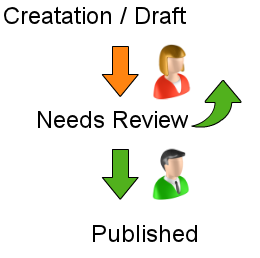
\includegraphics{workflow_simple.png}\hfill}


\section{Expanded Workflow}
\label{workbench:expanded-workflow}
Adding a publisher lets us look at how to define new states, transitions, and views.

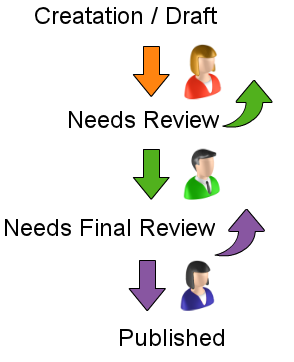
\includegraphics{workflow.png}


\section{Ingredients}
\label{workbench:ingredients}

\subsection{Staple}
\label{workbench:staple}\begin{enumerate}
\item {} 
\href{http://drupal.org/project/ctools}{http://drupal.org/project/ctools} - Enable Chaos tools

\item {} 
\href{http://drupal.org/project/views}{http://drupal.org/project/views} - Views: Enable Views and Views UI

\item {} 
\href{http://drupal.org/project/workbench}{http://drupal.org/project/workbench} - Enable Workbench

\item {} 
\href{http://drupal.org/project/workbench\_moderation}{http://drupal.org/project/workbench\_moderation} - Enable Workbench Moderation

\item {} 
\href{http://drupal.org/project/diff}{http://drupal.org/project/diff} - Enable Diff

\end{enumerate}

\textbf{Drush users:}

\begin{Verbatim}[commandchars=\\\{\}]
drush dl ctools views workbench workbench\_moderation diff
drush en ctools views workbench workbench\_moderation -y
\end{Verbatim}


\section{Part 1: Users and permissions}
\label{workbench:part-1-users-and-permissions}
\emph{People \textgreater{} Permissions}

We're working with three pre-created users, each of whom is assigned to one of the three pre-created roles that will be used in the workflow. Creating users and roles is routine, but permissions are one of the trickiest things to get right when creating a workflow, so we're working through that together.
\begin{figure}[htbp]
\centering
\capstart


\includegraphics{contributor.png}
\caption{Cathy Contributor}{\small 
Cathy has been assigned the Contributor role so that she will be able to create and edit her own content.
}\end{figure}
\begin{figure}[htbp]
\centering
\capstart


\includegraphics{editor.png}
\caption{Eli Editor}{\small 
Eli has been assigned the Editor role so that in addition to being able to do anything a contributor can do, he will be able to edit the work of others and advance content for publication.
}\end{figure}
\begin{figure}[htbp]
\centering
\capstart


\includegraphics{publisher.png}
\caption{Peggy Publisher}{\small 
Peggy has been assigned the Publisher role. This is the only role that will be able to make content live on the site. Publishers can do everything that editors and contributors can do.
}\end{figure}


\subsection{1.1: Node permissions}
\label{workbench:node-permissions}
Before setting up the second layer of permissions provided by Workbench Moderation, we'll set the basic node permissions. These settings are based on the premise that no site content is ever deleted. During development, you might choose to allow the deletion of content.

\begin{tabulary}{\linewidth}{|L|L|L|L|}
\hline
\textbf{
Permission
} & \textbf{
Contributor
} & \textbf{
Editor
} & \textbf{
Publisher
}\\\hline

View own unpublished content
 & 
{[}√{]}
 & 
{[}√{]}
 & 
{[}√{]}
\\\hline

View content revisions
 & 
{[}√{]}
 & 
{[}√{]}
 & 
{[}√{]}
\\\hline

Revert content revisions
 & 
{[} {]}
 & 
{[}√{]}
 & 
{[}√{]}
\\\hline

Delete content revisions
 & 
{[} {]}
 & 
{[} {]}
 & 
{[} {]}
\\\hline

Article: Create new content
 & 
{[}√{]}
 & 
{[}√{]}
 & 
{[}√{]}
\\\hline

Article: Edit own content
 & 
{[}√{]}
 & 
{[}√{]}
 & 
{[}√{]}
\\\hline

Article: Edit any content
 & 
{[} {]}
 & 
{[}√{]}
 & 
{[}√{]}
\\\hline

Article: Delete own content
 & 
{[} {]}
 & 
{[} {]}
 & 
{[} {]}
\\\hline

Article: Delete any content
 & 
{[} {]}
 & 
{[} {]}
 & 
{[} {]}
\\\hline

Basic page: Create new content
 & 
{[}√{]}
 & 
{[}√{]}
 & 
{[}√{]}
\\\hline

Basic page: Edit own content
 & 
{[}√{]}
 & 
{[}√{]}
 & 
{[}√{]}
\\\hline

Basic page: Edit any content
 & 
{[} {]}
 & 
{[}√{]}
 & 
{[}√{]}
\\\hline

Basic page: Delete own content
 & 
{[}√{]}
 & 
{[} {]}
 & 
{[}√{]}
\\\hline

Basic page: Delete any content
 & 
{[} {]}
 & 
{[} {]}
 & 
{[}√{]}
\\\hline
\end{tabulary}



\section{Part 2: Configure workbench moderation}
\label{workbench:part-2-configure-workbench-moderation}

\subsection{2.1: Review configuration}
\label{workbench:review-configuration}
\emph{Configuration \textgreater{} Workbench: Workbench Moderation}

We will start by using the default states provided by Workbench Moderation and later add new ones. The labeling of states is tricky business since the contributor chooses a state before it's been applied and everyone else sees the state afterward. In general, it's best to choose the label that makes the most sense \emph{after} it has been applied, e.g., Published instead of Publish.


\subsection{2.2: Enable the workflow for content types}
\label{workbench:enable-the-workflow-for-content-types}
\emph{Structure \textgreater{} Content types \textgreater{} Article: edit}

Although we don't cover this today, it is possible to have different workflows for different content types. This gets complex very quickly! See \href{http://drupal.org/node/1206854\#comment-5241230}{http://drupal.org/node/1206854\#comment-5241230} for how to enable this.
\begin{enumerate}
\item {} 
Publishing options

\item {} 
{[} {]} Published (Uncheck this)

\item {} 
{[}√{]} Promoted to front page (Leave checked)

\item {} 
{[} {]} Sticky at top of lists (Leave unchecked)

\item {} 
{[}√{]} Create a new revision (Check this!)

\item {} 
{[}√{]} Enable moderation of revisions (Can only be checked once the item above is checked. Check this).

\item {} 
Default moderation state: Draft

\item {} 
Save content type

\item {} 
Repeat for the Basic page content type (although don't promote pages to the front page)

\end{enumerate}


\subsection{2.3: Set the Workbench Moderation permissions}
\label{workbench:set-the-workbench-moderation-permissions}
\emph{People \textgreater{} Permissions}

At the bottom of the modules page:

\textbf{Workbench}

\begin{tabulary}{\linewidth}{|L|L|L|L|}
\hline
\textbf{
Permission
} & \textbf{
Contributor
} & \textbf{
Editor
} & \textbf{
Publisher
}\\\hline

Administer Workbench settings
 & 
{[} {]}
 & 
{[} {]}
 & 
{[} {]}
\\\hline

Access My Workbench
 & 
{[}√{]}
 & 
{[}√{]}
 & 
{[}√{]}
\\\hline
\end{tabulary}


\textbf{Workbench Moderation}

\begin{tabulary}{\linewidth}{|L|L|L|L|}
\hline
\textbf{
Permission
} & \textbf{
Contributor
} & \textbf{
Editor
} & \textbf{
Publisher
}\\\hline

View all unpublished content
 & 
{[} {]}
 & 
{[}√{]}
 & 
{[}√{]}
\\\hline

Administer Workbench Moderation
 & 
{[} {]}
 & 
{[} {]}
 & 
{[} {]}
\\\hline

Bypass moderation restrictions
 & 
{[} {]}
 & 
{[} {]}
 & 
{[} {]}
\\\hline

View moderation history
 & 
{[}√{]}
 & 
{[}√{]}
 & 
{[}√{]}
\\\hline

View the moderation messages on a node
 & 
{[}√{]}
 & 
{[}√{]}
 & 
{[}√{]}
\\\hline

Use ``My Drafts'' workbench tab
 & 
{[}√{]}
 & 
{[}√{]}
 & 
{[}√{]}
\\\hline

Use ``Needs Review'' workbench tab
 & 
{[} {]}
 & 
{[}√{]}
 & 
{[}√{]}
\\\hline

Moderate all content from Draft to Needs Review*
 & 
{[}√{]}
 & 
{[}√{]}
 & 
{[}√{]}
\\\hline

Moderate all content from  Needs Review to Draft
 & 
{[} {]}
 & 
{[}√{]}
 & 
{[}√{]}
\\\hline

Moderate all content from Needs Review to Published
 & 
{[} {]}
 & 
{[}√{]}
 & 
{[}√{]}
\\\hline
\end{tabulary}

\begin{itemize}
\item {} 
It's oddly worded, but you must grant this permission to the Contributor. It really means ``Moderate all content types to Needs review.'' It is limited in scope by your particular permissions for each content type. The Contributor role is only allowed to edit its own Articles and Basic Pages, so it Cathy Contributor won't be able to Moderate other peoples' work.

\end{itemize}


\subsection{2.4 Check your permissions}
\label{workbench:check-your-permissions}
{\color{red}\bfseries{}*}Configuration \textgreater{} Workbench: Workbench Moderation \textgreater{} Check permissions (tab)

Workbench has a great feature to help ensure you've set up your transitions properly.


\section{Part 3: Watch Contributor \textgreater{} Editor Moderation in Action}
\label{workbench:part-3-watch-contributor-editor-moderation-in-action}
\emph{Home}

We're going to set up in two separate browsers, once for Cathy Contributor and one for Eli Editor so that we can watch as content progresses through the workflow.


\subsection{3.1: Create an article as Cathy Contributor}
\label{workbench:create-an-article-as-cathy-contributor}\begin{figure}[htbp]
\centering


\includegraphics{contributor.png}
{\small \begin{enumerate}
\item {} 
In the first browser, log in as admin and masquerade as Cathy Contributor.

\item {} 
Create a new article.

\item {} 
Note the message that the draft will be placed in moderation.

\end{enumerate}
}\end{figure}


\subsection{3.2: View Eli Editor's Worbench}
\label{workbench:view-eli-editor-s-worbench}
\emph{My Workbench \textgreater{} Needs Review (tab)}
\begin{figure}[htbp]
\centering


\includegraphics{editor.png}
{\small \begin{enumerate}
\item {} 
In the second browser, log in as admin and masquerade as Eli Editor.

\item {} 
View My Workbench \textgreater{} Needs Review (tab)

\item {} 
You shouldn't see anything yet.

\end{enumerate}
}\end{figure}


\subsection{3.3: Move Cathy's work to Needs Review}
\label{workbench:move-cathy-s-work-to-needs-review}
Workbench \textgreater{} My Drafts*
\begin{figure}[htbp]
\centering


\includegraphics{contributor.png}
{\small 
Cathy Contributor can move her work from Draft to Needs Review in three places:
\begin{itemize}
\item {} 
On the View draft tab of the node, just as soon as she's saved it

\item {} 
On the Moderate tab, where the entire revision history is available

\item {} 
From the My Drafts page

\end{itemize}

Her work will be visible to no one but an administrator until she moves it to the Needs Review state.
\begin{enumerate}
\item {} 
Move the article created in 2.4.1 into the Needs Review state.

\item {} 
Note that it disappears from Drafts and reappears on the My content page in My Edits. If Cathy bookmarks the page, she can still edit this while it's in the Needs review state, good for fixing that last typo.

\end{enumerate}
}\end{figure}


\subsection{3.4: Publish Cathy's article}
\label{workbench:publish-cathy-s-article}
\emph{My Workbench \textgreater{} Needs Review (tab)}
\begin{figure}[htbp]
\centering


\includegraphics{editor.png}
{\small \begin{enumerate}
\item {} 
Reload Eli Editor's Needs Review tab.

\item {} 
Locate Cathy's new article.

\item {} 
Publish it.

\end{enumerate}
}\end{figure}

What if you'd like to return the article to Cathy because it needs work? You can send it back by setting it to Draft, but out of the box, it's difficult to add a message to the page. We'll fix that as best we can in Part 5: Adjusting the Views. There is a feature request to make it easier to add comments at \href{http://drupal.org/node/1257650}{http://drupal.org/node/1257650}.


\subsection{3.5: As Cathy, review the published work}
\label{workbench:as-cathy-review-the-published-work}
\emph{My Workbench}
\begin{figure}[htbp]
\centering


\includegraphics{contributor.png}
{\small \begin{enumerate}
\item {} 
Take a look at Cathy's main workbench page.

\item {} 
Edit the Contributor FAQ

\item {} 
Note that the officially-approved content stays published while this draft goes into moderation.

\end{enumerate}
}\end{figure}


\subsection{3.6: Experiment}
\label{workbench:experiment}\begin{enumerate}
\item {} 
Try routing the article between Cathy and Eli in ways your organization might use workflow.

\item {} 
Try creating content as Eli.

\item {} 
Switch back to the admin account when you're done.

\end{enumerate}


\section{Part 4: Expanding the Workflow}
\label{workbench:part-4-expanding-the-workflow}

\subsection{4.1: Add a new state}
\label{workbench:add-a-new-state}
\emph{Configuration \textgreater{} Workbench: Workbench Moderation}

{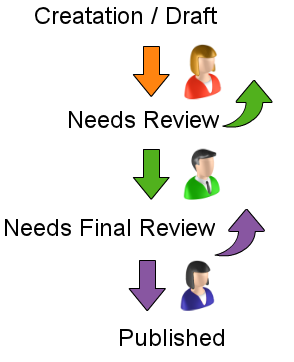
\includegraphics{workflow.png}\hfill}
\begin{enumerate}
\item {} 
On the main screen, add a state:

Name: Needs Final Review

Description: Ready for Publication

\item {} 
Arrange them in order by using the grabber.
\begin{itemize}
\item {} 
Draft

\item {} 
Needs Review

\item {} 
Needs Final Review

\item {} 
Published

\end{itemize}

\item {} 
Save

\end{enumerate}

When you save, you'll see the following warning: Depending on the changes you have made it may be necessary to reconfigure Views that leverage Workbench Moderation such as workbench\_moderation. Part 5 will address the customizations necessary to take advantage of our new state.


\subsection{4.2: Enable the transitions}
\label{workbench:enable-the-transitions}
\emph{Configuration \textgreater{} Workbench: Workbench Moderation: Transitions (tab)}

Next we define the new transitions. Move to the Transitions tab and:
\begin{enumerate}
\item {} 
Add Needs Review \textgreater{} Needs Final Review
This will let us give editors permission to advance content to publishers.

\item {} 
Add Needs Final Review \textgreater{} Needs Review
This will allow us to give publishers the ability to send the content back to the editors.

\item {} 
Add Needs Final Review \textgreater{} Published
This will allow us to give the publisher permission to publish.

\item {} 
Delete Needs Review \textgreater{} Published
This will removes an editor's ability to publish without final review.

\end{enumerate}


\subsection{4.3: Assign transition permissions}
\label{workbench:assign-transition-permissions}
\emph{People \textgreater{} Permissions}

Set the new permissions.

\textbf{Workbench Moderation}

\begin{tabulary}{\linewidth}{|L|L|L|L|}
\hline
\textbf{
Permission
} & \textbf{
Contributor
} & \textbf{
Editor
} & \textbf{
Publisher
}\\\hline

Moderate all content from Needs Review to Needs Final Review
 & 
{[} {]}
 & 
{[}√{]}
 & 
{[}√{]}
\\\hline

Moderate all content from Needs Final Review to Needs Review
 & 
{[} {]}
 & 
{[} {]}
 & 
{[}√{]}
\\\hline

Moderate all content from Needs Final Review to Published
 & 
{[} {]}
 & 
{[} {]}
 & 
{[}√{]}
\\\hline
\end{tabulary}



\section{Part 5: Adjust the views}
\label{workbench:part-5-adjust-the-views}
\emph{Structure \textgreater{} Views \textgreater{} workbench\_moderation: edit}

Since we added our own state, we'll need to create another tab that is visible to the Publisher.
\begin{enumerate}
\item {} 
Select the display: Needs Review Page

\item {} 
Clone it

\item {} 
Display Name: Ready to Publish Page

\item {} 
Title: Ready to Publish

\item {} 
Filter Criteria \textgreater{} Workbench Moderation State: Needs Final Review

\item {} 
Page Settings \textgreater{} Path: admin/workbench/ready-to-publish

\item {} 
Page Settings \textgreater{} Menu \textgreater{} Title: Ready to Publish

\item {} 
Page Settings \textgreater{} Access: Permissions (change to role and select Publisher)

\end{enumerate}


\section{Part 6: Watch Editor \textgreater{} Publisher Moderation in Action}
\label{workbench:part-6-watch-editor-publisher-moderation-in-action}

\subsection{6.1: Create an article as Eli Editor}
\label{workbench:create-an-article-as-eli-editor}
\emph{Home}
\begin{figure}[htbp]
\centering


\includegraphics{editor.png}
{\small \begin{enumerate}
\item {} 
In the first browser, log in as admin and masquerade as Eli Editor.

\item {} 
Create a new article
Title: Editorial Policies
Body:  Just because you \emph{can} move your work without review by another editor may not mean you should.

\item {} 
Save

\item {} 
Move it directly to Needs Final Review

\end{enumerate}
}\end{figure}


\subsection{6.2: View Peggy Publisher's Workbench}
\label{workbench:view-peggy-publisher-s-workbench}
\emph{My Workbench \textgreater{} Needs Review (tab)}
\begin{figure}[htbp]
\centering


\includegraphics{publisher.png}
{\small \begin{enumerate}
\item {} 
In the second browser, log in as adhttp://workflow.everydaydrupal.com/min and masquerade as Peggy Publisher.

\item {} 
View My Workbench \textgreater{} Ready for Publication (tab)

\item {} 
Publish Eli's Editorial Policies article.

\end{enumerate}
}\end{figure}


\subsection{6.3: Move Eli's work to Needs Review}
\label{workbench:move-eli-s-work-to-needs-review}
\emph{My Workbench \textgreater{} My Drafts}


\subsection{Part 7: Design your own workflow}
\label{workbench:part-7-design-your-own-workflow}
Extend your understanding by working on one of the following:

If this workflow is exactly what you need, consider:
\begin{enumerate}
\item {} 
How could the workbench moderation pages do a better job of supporting the process in your organization?

\item {} 
What additional features might you want?

\end{enumerate}

If this workflow doesn't meet your needs, design one that does.


\chapter{Keeping it Fresh: Scheduling Content}
\label{schedule:keeping-it-fresh-scheduling-content}\label{schedule::doc}
Intro blurb


\section{Ingredients}
\label{schedule:ingredients}

\subsection{Staple}
\label{schedule:staple}\begin{enumerate}
\item {} 
\href{http://drupal.org/project/ctools}{http://drupal.org/project/ctools} Enable Chaos Tools

\item {} 
\href{http://drupal.org/project/views}{http://drupal.org/project/views} Enable Views and Views UI

\item {} 
\href{http://drupal.org/project/date}{http://drupal.org/project/date} Enable Date and Date Popup

\item {} 
\href{http://drupal.org/project/scheduler}{http://drupal.org/project/scheduler} Enable Scheduler

\item {} 
\href{http://drupal.org/project/diff}{http://drupal.org/project/diff} Enable Diff

\end{enumerate}


\section{Part 1: Create content to work with}
\label{schedule:part-1-create-content-to-work-with}
\emph{Configuration \textgreater{} Development: Generate Content}
\begin{enumerate}
\item {} 
{[}√{]} Check Article

\item {} 
{[} {]} Uncheck Basic Page

\item {} 
Generate 50 articles, going back in time for a year.

\item {} 
Generate

\end{enumerate}


\section{Part 2: The latest content approach}
\label{schedule:part-2-the-latest-content-approach}
\emph{Structure \textgreater{} Views \textgreater{} +Add a new view}

Pros: Content is still visible if a user reaches it via a link from elsewhere or a search engine.

Cons: The article is still visible. :)


\section{Part 3: Schedule articles}
\label{schedule:part-3-schedule-articles}


\renewcommand{\indexname}{Index}
\printindex
\end{document}
